\chapter{The Standard Model, Supersymmetry, and the motivations behind it}
\label{ch:theory} 
\epigraph{\emph{A theory is something nobody believes, except the person who made it. An experiment is something everybody believes, except the person who made it.}} {Albert Einstein}

	The Standard Model (SM) of particle physics is an effective theory that aims to provide a general description of fundamental particles and the phenomena we see in nature, \ie\ the way they interact. Unfortunately, our understanding of nature is still limited due to some opened question to which the SM is not able to answer to, yet. 

	In this chapter, an overview of the SM will be presented in Section \ref{sec:SMov} together with the limitations of such theory and some of the reasons behind the need of an extension. For the last decades theoretical physicsts have been trying to provide extensions to the SM, the so-called beyond-the-SM theories. Among these, one of the most popular, Supersymmetry which will be discussed in Section \ref{sec:SUSY}.  

	
	


	\section{Overview}
	%\label{sec:SM}
	\label{sec:SMov}

		The 20$^{th}$ century can be considered a quantum revolution. Several experiments led to discoveries which were found to be, together with the formalised theory, a solid base of the Standard Model of particle physics and our description of nature. Several particles were predicted first by the SM and then experimentally observed \eg\ the \Wboson\ and the \Zboson\ bosons, the $\tau$ lepton, \cite{Herrero1998}, and more recently the Higgs boson at the LHC discovered by ATLAS \cite{ATLASHiggs2012} and CMS \cite{CMSHiggs2012}.

		The SM lays on a Quantum Field Theory (QFT) where particles are treated like fields. It can describe three of the four fundamental forces; weak, electromagnetic, and strong. As of today, gravity is not considered in the SM. Sections \ref{sec:SMov} and \ref{sec:SMlim} will be focused on the description of the fields together with the carriers of the information, and on the limitations that such theory implies, respectively.


	% \subsection{Overview}
	% \label{sec:SMov}

		The most general classification of the particles within the SM can be made by means of spin. Fermions have half-integer spin values - and are usually referred to as matter -, and bosons have integer-spin values. A noteworthy subset of bosons is formed by the Spin-1 bosons (also known as gauge bosons). These can be considered the information carriers or, in fact, the mediators of the forces. 



		\subsection*{Fermions}

			Six quarks and six leptons belong to the fermions family. In particular, fermions can be grouped into three generations. Each generation contains four particles; one up- and one down-type quark, one charged lepton and one neutral lepton. The masses of the charged leptons and quarks increase with the generation. The six quarks of the SM can be grouped into three doublets:

			\begin{equation*}
			\label{eq:quark_doublets}
				\begin{pmatrix} u \\ d \end{pmatrix}, \qquad 
				\begin{pmatrix} c \\ s \end{pmatrix}, \qquad 
				\begin{pmatrix} t \\ b \end{pmatrix}
			\end{equation*}

			\noindent The up-type quarks (up, charm, top) have charge $+\frac{2}{3}e$ and the down-type quarks (down, strange, beauty/bottom) have charge $-\frac{1}{3}e$, where $e$ is the electron charge. Quarks also have another quantum number that can be seen as the analogue of the electric charge, which is the colour charge. This can exist in three different states; ``red'', ``green'' and ``blue''. Moreover, as a consequence of \emph{confinement}, which will be discussed later on in this section, quarks cannot exist as free particles. They rather group to form hadronic matter, also known as \emph{hadrons}. There are two kinds of hadrons; mesons and baryons. Mesons are quark-antiquark systems, \eg the pion, and baryons are three-quark system, \eg protons and neutrons. Quarks and anti-quarks have a baryon number of $\frac{1}{3}$ and $-\frac{1}{3}$, respectively.

			There are six leptons and they can be classified in charged leptons (electron $e$, muon $\mu$, tau $\tau$) and neutral leptons (electron neutrino $\nu_e$, muon neutrino $\nu_{\mu}$, tau neutrino $\nu_{\tau}$).

			%\noindent Generations are classified according to the state of chirality, which is a non-physical concept close enough to helicity which, in turn, is the projection of the spin onto the direction of momentum. Chirality is equivalent to helicity for massless particles and, as per helicity states, there can either be left-handed chiral states or right-handed chiral states.
			
			\begin{equation*}
			\label{eq:lepton_flavor_doublets}
				\begin{pmatrix} \nu_e      \\ e^-    \end{pmatrix}, \qquad
				\begin{pmatrix} \nu_{\mu}  \\ \mu^-  \end{pmatrix}, \qquad
				\begin{pmatrix} \nu_{\tau} \\ \tau^- \end{pmatrix}
			\end{equation*}

			\noindent Each lepon has a charachteristic quantum number, called lepton number ($L$). Negatively (positively) charged leptons have $L=-1$ ($L=1$) and neutral leptons have $L=0$. The lepton number is conserved in all the interactions. 



		\subsection*{Forces of Nature}

			Forces in the SM are described by gauge theories, where the interactions is mediated by a vector gauge boson. 

			The electromagnetic force is described by Quantum ElectroDynamics (QED) and, as its mediator is the photon ($\gamma$) which couples to charged particles, it only affects charged leptons and quarks, not neutrinos. They are instead affected by the weak force which is mediated by the bosons $\Wboson^{\pm}$ and $\Zboson^0$. 

			The weak interaction is associated with handedness (the projection of a particle spin onto its direction of motion). Both leptons and quarks have left- and right-handed components. However, only the left-handed (right-handed) component for neutrinos (anti-neutrinos) has been observed. This means that nature prefers to produce left-handed neutrinos and right-handed anti-neutrinos, which is the so-called parity violation. 

			The strong interactions, mediated by the gluon (electrically neutral and massless), is described by Quantum ChromoDynamics (QCD). Its coupling increases with increasing distance and is smaller at short range. Moreover, due to gluon self interactions, two different phenomena arise; \emph{confinement}: neither quarks nor gluons are observed as free particles, but only colourless “singlet” states can be observed as “jets”, namely collimated cone-shaped sprays of hadrons; \emph{asymptotic freedom}: interactions between quarks and gluons become weaker as the energy scale increases and the corresponding length scale decreases.

			Table \ref{tab:interactions} summarises the forces described in the SM and their mediators' main charachteristics. Finally, the gravitational force, which is believed to be mediated by the graviton, is not included in Table \ref{tab:interactions} as it is not part of the SM.

			\begin{table}[!htb]\centering\caption{Forces and mediators described by the SM}							
				\begin{tabular}{c|c|c|c|c}
					\hline \hline
					Force & Name & Symbol & Mass [\GeV]& Charge \\ \hline \hline
					Electromagnetic & Photon & $\gamma$ & 0 & 0 \\ \hline
					\multirow{2}{*}{Weak} & W & $\Wboson^{\pm}$ & $80.398$ & $\pm e$ \\
					& Z & $\Zboson^0$ & $91.188$ & 0 \\\hline
					Strong & Gluon & $g$ & $0$ & $0$ \\\hline\hline
				\end{tabular}						
			\label{tab:interactions} 
			\end{table}



		\subsection*{Symmetries and Gauge Groups}

			In 1915, the mathematician Emmy Noether (23 March 1882 – 14 April 1935) proved that every differentiable symmetry of the action - defined as the integral over space of a Lagrangian density function - of a physical system has a corresponding conservation law. More generally, a symmetry is a property of a physical system. Under certain transformations this property is preserved. 

			A gauge theory in QFT, is a theory in which the Lagrangian is invariant under a continuous group of local transformation. Group theory was then adopted to describe the symmetries conserved in the SM.  
			%The term gauge is related to the mathematical formalism that regulates redundant degrees of freedom in the Lagrangian. 
			The gauge group of the theory is the \emph{Lie Group}. It contains all the transformations between possible gauges. The Lie algebra of group generators is therefore associated with any Lie group and for each group generator there emerges a corresponding field: the gauge field. The quanta of the gauge fields are called \emph{gauge bosons}.
			%To ensure the invariance of the SM Lagrangian under the local group transformations, gauge fields are included. 
			
			The three SM interactions can therefore be mathematically described by the following:

			\begin{equation}
			\label{eq:SM_gaugeSym}
				U(1)_Y \otimes SU(2)_L \otimes SU(3)_C
			\end{equation}

			\noindent Here, $Y$ is the weak hypercharge, used to estimate the correlation between the electric charge ($Q$) and the third component of the weak isospin ($I_3$) via the relation $Q = I_3 + Y/2$, where $I_3$ can either be $\pm 1/2$ or $0$ for left-handed and right-handed particles, respectively; $C$ the colour charge and $L$ the left-handedness. 

			As of today, we can describe three of the four forces of nature with group theory. QED is an Abelian gauge theory with $U(1)$ as symmetry group, with the electromagnetic four-potential as its gauge field and with the photon as its gauge boson \cite{Pich2012}. The interactions between charged fermions occurs by the exchange of a massless photon. 

			The weak interaction and the strong interactions are non-Abelian gauge theories with gauge groups $SU(2)$ and $SU(3)$, respectively. As a consequence of being non-Abelian the generators commutators are non-vanishing and therefore the gauge bosons can self-interact. The $SU(2)$ generators of the weak interaction are the massless gauge bosons $W_{\mu}^{\alpha = 1,\dots,3}$ and, as mentioned earlier on in this chapter, they violate the parity by acting only on left-handed particles. 

			The gauge bosons of $SU(3)_C$ are eight massless gluons, $G_{\mu}^{\alpha=1,\dots,8}$. The strong interaction does not distinguish left- and right-handed particles. 
			Finally, the Quarks that interact through weak interaction are mixtures of SM eigenstates as described by the CKM matrix \cite{Olive2014}.



		\subsection*{Electroweak Symmetry Breaking and the Higgs mechanism}

			In 1979 Sheldon Glashow, Abdus Salam, and Steven Weinberg were awarded the Nobel Prize in Physics for their contributions to the so-called electroweak unification. In the mathematical description of the SM in \ref{eq:SM_gaugeSym} the electroweak interaction is described by $U(1)_Y \otimes SU(2)_L$. The electroweak physical bosons \Wboson, \Zboson\ and $\gamma$ are related to the four unphysical gauge bosons $W_{\mu}^{\alpha = 1,\dots,3}$ and $B_\mu^0$. In particular, to obtain the physical bosons the gauge bosons have to mix as follows:

			\begin{equation}
			\label{eq:mixing}
					\begin{pmatrix} A_{\mu} \\ Z_{\mu} \end{pmatrix}					
					= 
					\begin{pmatrix}
							\cos\theta_W & \sin\theta_W \\ 
							-\sin\theta_W & \cos\theta_W
						\end{pmatrix}
					\begin{pmatrix}
						B_{\mu} \\ W_{\mu}^3
						\end{pmatrix}
			\end{equation}

			Here, $\theta_W$ is the so-called \emph{Weinberg angle} which is the angle by which spontaneous symmetry breaking rotates the original $\Wboson_{\mu}^3$ and $B_{\mu}$, producing the physical \Zboson, and the photon. $\theta_W$ can be experimentally determined in terms of the coupling strengths of the $B_{\mu}(g_1)$ and the $W_{\mu}^\alpha (g_2)$ to the fermions using the relation $\tan\theta_W = g_1 / g_2 $. The field mixing of gauge bosons that gives birth to the physical ones can be mathematically expressed by the following:

			\begin{equation}
			\label{eq:photon}
				A_{\mu} = W_{\mu}^3 \sin\theta_W  + B_{\mu}\cos \theta_W 
			\end{equation}
			\begin{equation}
			\label{eq:Zboson}
				Z_{\mu} = W_{\mu}^3\cos\theta_W  - B_{\mu} \sin \theta_W
			\end{equation}

			\noindent where $A_\mu$ and $Z_\mu$ represent the photon and the \Zboson\ boson, respectively. The charged vector bosons, $W_\mu^\mp$, and its complex conjugate are defined as:

			\begin{equation}
			\label{eq:Wboson}
				W_{\mu}^\pm = \frac{1}{\sqrt{2}} \displaystyle \left ( W_{\mu}^1 \mp i W_{\mu}^2 \right )
			\end{equation}

			Mass terms for both gauge bosons and fermionic fields are not invariant under gauge transformations and are therefore forbidden by the electroweak gauge. Nonetheless, it is proven by experiments that \Wboson\ and \Zboson\ are massive \cite{Pich2012}, therefore the SM assumption only holds if the electroweak symmetry is broken. 

			The SM Lagrangian can be written as the sum of the various Lagrangians describing the three interactions and the masses of the elementary particles as follows:

			\begin{equation}
			\label{eq:SM_Lagrangian}
				\mathcal{L_{\mathrm{SM}}} = \mathcal{L_{\mathrm{EWK}}} + \mathcal{L_{\mathrm{QCD}}} + \mathcal{L_{\mathrm{Mass}}}
			\end{equation}

			\noindent In order for the SM Lagrangian to remain a renormalisable theory, mass terms ($\mathcal{L_{\mathrm{Mass}}}$) cannot be insterted by hand. A mechanism, that can preserve the gauge symmetry in the SM and, that can solve the inconsistency arisen from the mass difference between the gauge bosons and the physical ones, is needed. A British theoretical physicist, Peter Higgs (29 May 1929, Newcastle upon Tyne, UK), came up with a brilliant solution for which he was awarded the 2013 Physics Nobel Prize. In the 1960s, Higgs proposed that broken symmetry in electroweak theory could explain the origin of masses of elementary particles, and in particular of \Wboson\ and \Zboson\ bosons: the Higgs mechanism was given birth. % and with it the Higgs Lagrangian in Eq. \ref{eq:Higgs_lagrangian}.
			The mechanism introduces a scalar field, known as the Higgs field, thought to couple to both massive fermions and bosons. 

			In the SM the Higgs field is a doublet in $SU(2)$:
			\begin{equation}
				\phi = 
				\begin{pmatrix}
					\phi^+ \\ \phi^0
				\end{pmatrix} 
			\end{equation}

			\noindent with $\phi^+$ and $\phi^0$ being generic complex fields: 
			%This can be generally written as follows: %\cite{Englert1964, Higgs1964, Kibble1967}:

			\begin{equation}
				\phi^+ = \frac{\phi_1 + i \phi_2}{\sqrt{2}},  \qquad \phi^0 = \frac{\phi_3 + i \phi_4}{\sqrt{2}}
			\end{equation}

			Consider a Lagrangian of the form: 

			\begin{equation}
			\label{eq:Higgs_lagrangian}
				\mathcal{L_{\mathrm{Higgs}}} = ( \partial_{\mu} \phi )^* \left ( \partial^{\mu} \phi \right ) - V(\phi)
			\end{equation}

			\noindent Renormalizability and $SU(2)_L \otimes U(1)_Y$ invariance require the Higgs potential to be of the following form: 

			\begin{equation}
			\label{eq:Higgs_potential}
				V(\phi) = \mu^2  \phi^\dagger \phi + \lambda \left ( \phi^\dagger \phi \right )^2 
			\end{equation}

			\noindent Eq. \ref{eq:Higgs_lagrangian} is the Higgs Lagrangian if $\phi$ is chosen to be the following:

			\begin{equation*}
				\phi = 
				\begin{pmatrix}
					\phi^+ \\ \phi^0
				\end{pmatrix} 
				=
				\begin{pmatrix}
					G^+ \\ \frac{1}{\sqrt{2}} \left ( v + H + iG^0 \right )
				\end{pmatrix}
			\end{equation*}

			\noindent Here, the complex scalar field $G^\pm$ and the real scalar field $G^0$ correspond to Goldstone bosons, and the real scalar field $H$ is the SM Higgs boson field \cite{Goldstone1962}. These massless scalars are absorbed due to the gauge transformations by the electroweak gauge bosons of the SM:

			\begin{equation}
			\label{eq:Higgs_doublet}
				\phi = 
				\begin{pmatrix}
					\phi^+ \\ \phi^0
				\end{pmatrix} 
				=
				\begin{pmatrix}
					0 \\ \frac{1}{\sqrt{2}} \left ( v + H \right )
				\end{pmatrix}
			\end{equation}

			The Higgs potential in Eq. \ref{eq:Higgs_potential} is displayed in Fig. \ref{fig:higgs_potential} if $\lambda$ and $\mu$ are chosen to be real. Such potential has a non-zero ground state, $v$, also known as \emph{vacuum expectation value} (VEV):

			\begin{equation}
			\label{eq:Higgs_vev}
				\phi_0 = 
				\begin{pmatrix}
					0 \\ \frac{1}{\sqrt{2}} v
				\end{pmatrix}
			\end{equation}

			\noindent Such representation remains invariant under $U(1)$ allowing electric charge conservation. However, the SM gauge symmetry \ref{eq:SM_gaugeSym} is broken into $SU(2)_L \otimes U(1)_Y$.

			\begin{wrapfigure}{L}{.5\textwidth}
			\centering
				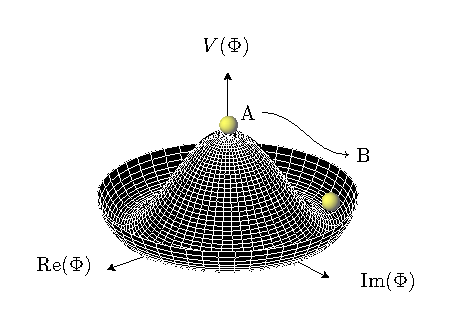
\includegraphics[width=.5\textwidth]{HiggsPotential/HiggsPotential}
			\caption{\label{fig:higgs_potential} The Higgs potential in the complex plane.} %Any given point around the bottom of the hat gives the lowest-energy state.}
			\end{wrapfigure}

			In summary, to generate particle masses gauge symmetry must be broken. However, in order for the theory to remain renormalisable, the global Lagrangian symmetry must be preserved. This can be solved introducing the concept of \emph{spontaneous} symmetry breaking (SSB): a mechanism that allows a symmetric Lagrangian, but not a symmetric VEV. In particular, given a Lagrangian invariant under a certain transformation, $T_X$ and a generic set of states, that transform under $T_X$ as the elements of a multiplet, the symmetry is spontaneously broken if one of those states is arbitrarily chosen as the ground state of the system. 
			%The Higgs-field VEV is not invariant under gauge transformations. In fact, it spontaneously breaks the gauge symmetry leaving the symmetry of the model untouched. 
			The interaction of the Higgs field with the $SU(2) \otimes U(1)$ gauge fields, $W_\mu^\alpha =1,2,3$, result in the three gauge bosons fields acquiring mass whilst the $B_0$ field stays massless. 





	\section{Limitations of the Standard Model}
	\label{sec:SMlim}

		During Run 1 and 2 of the LHC, the SM has been extensively validated, as shown in Fig. \ref{fig:ATLAS_a_SMSummary_TotalXsect}: the agreement, between the measured production cross section of various SM processes and the SM predictions, looks very good. However, the reasons behind the mass difference between the the three generations of fermions are still not explained by the SM because masses are treated as free parameters of the theory. In addition, there are some fundamental questions that have still no answer and they will be briefly discussed this section.

		\begin{figure}[!htb]
			\centering
			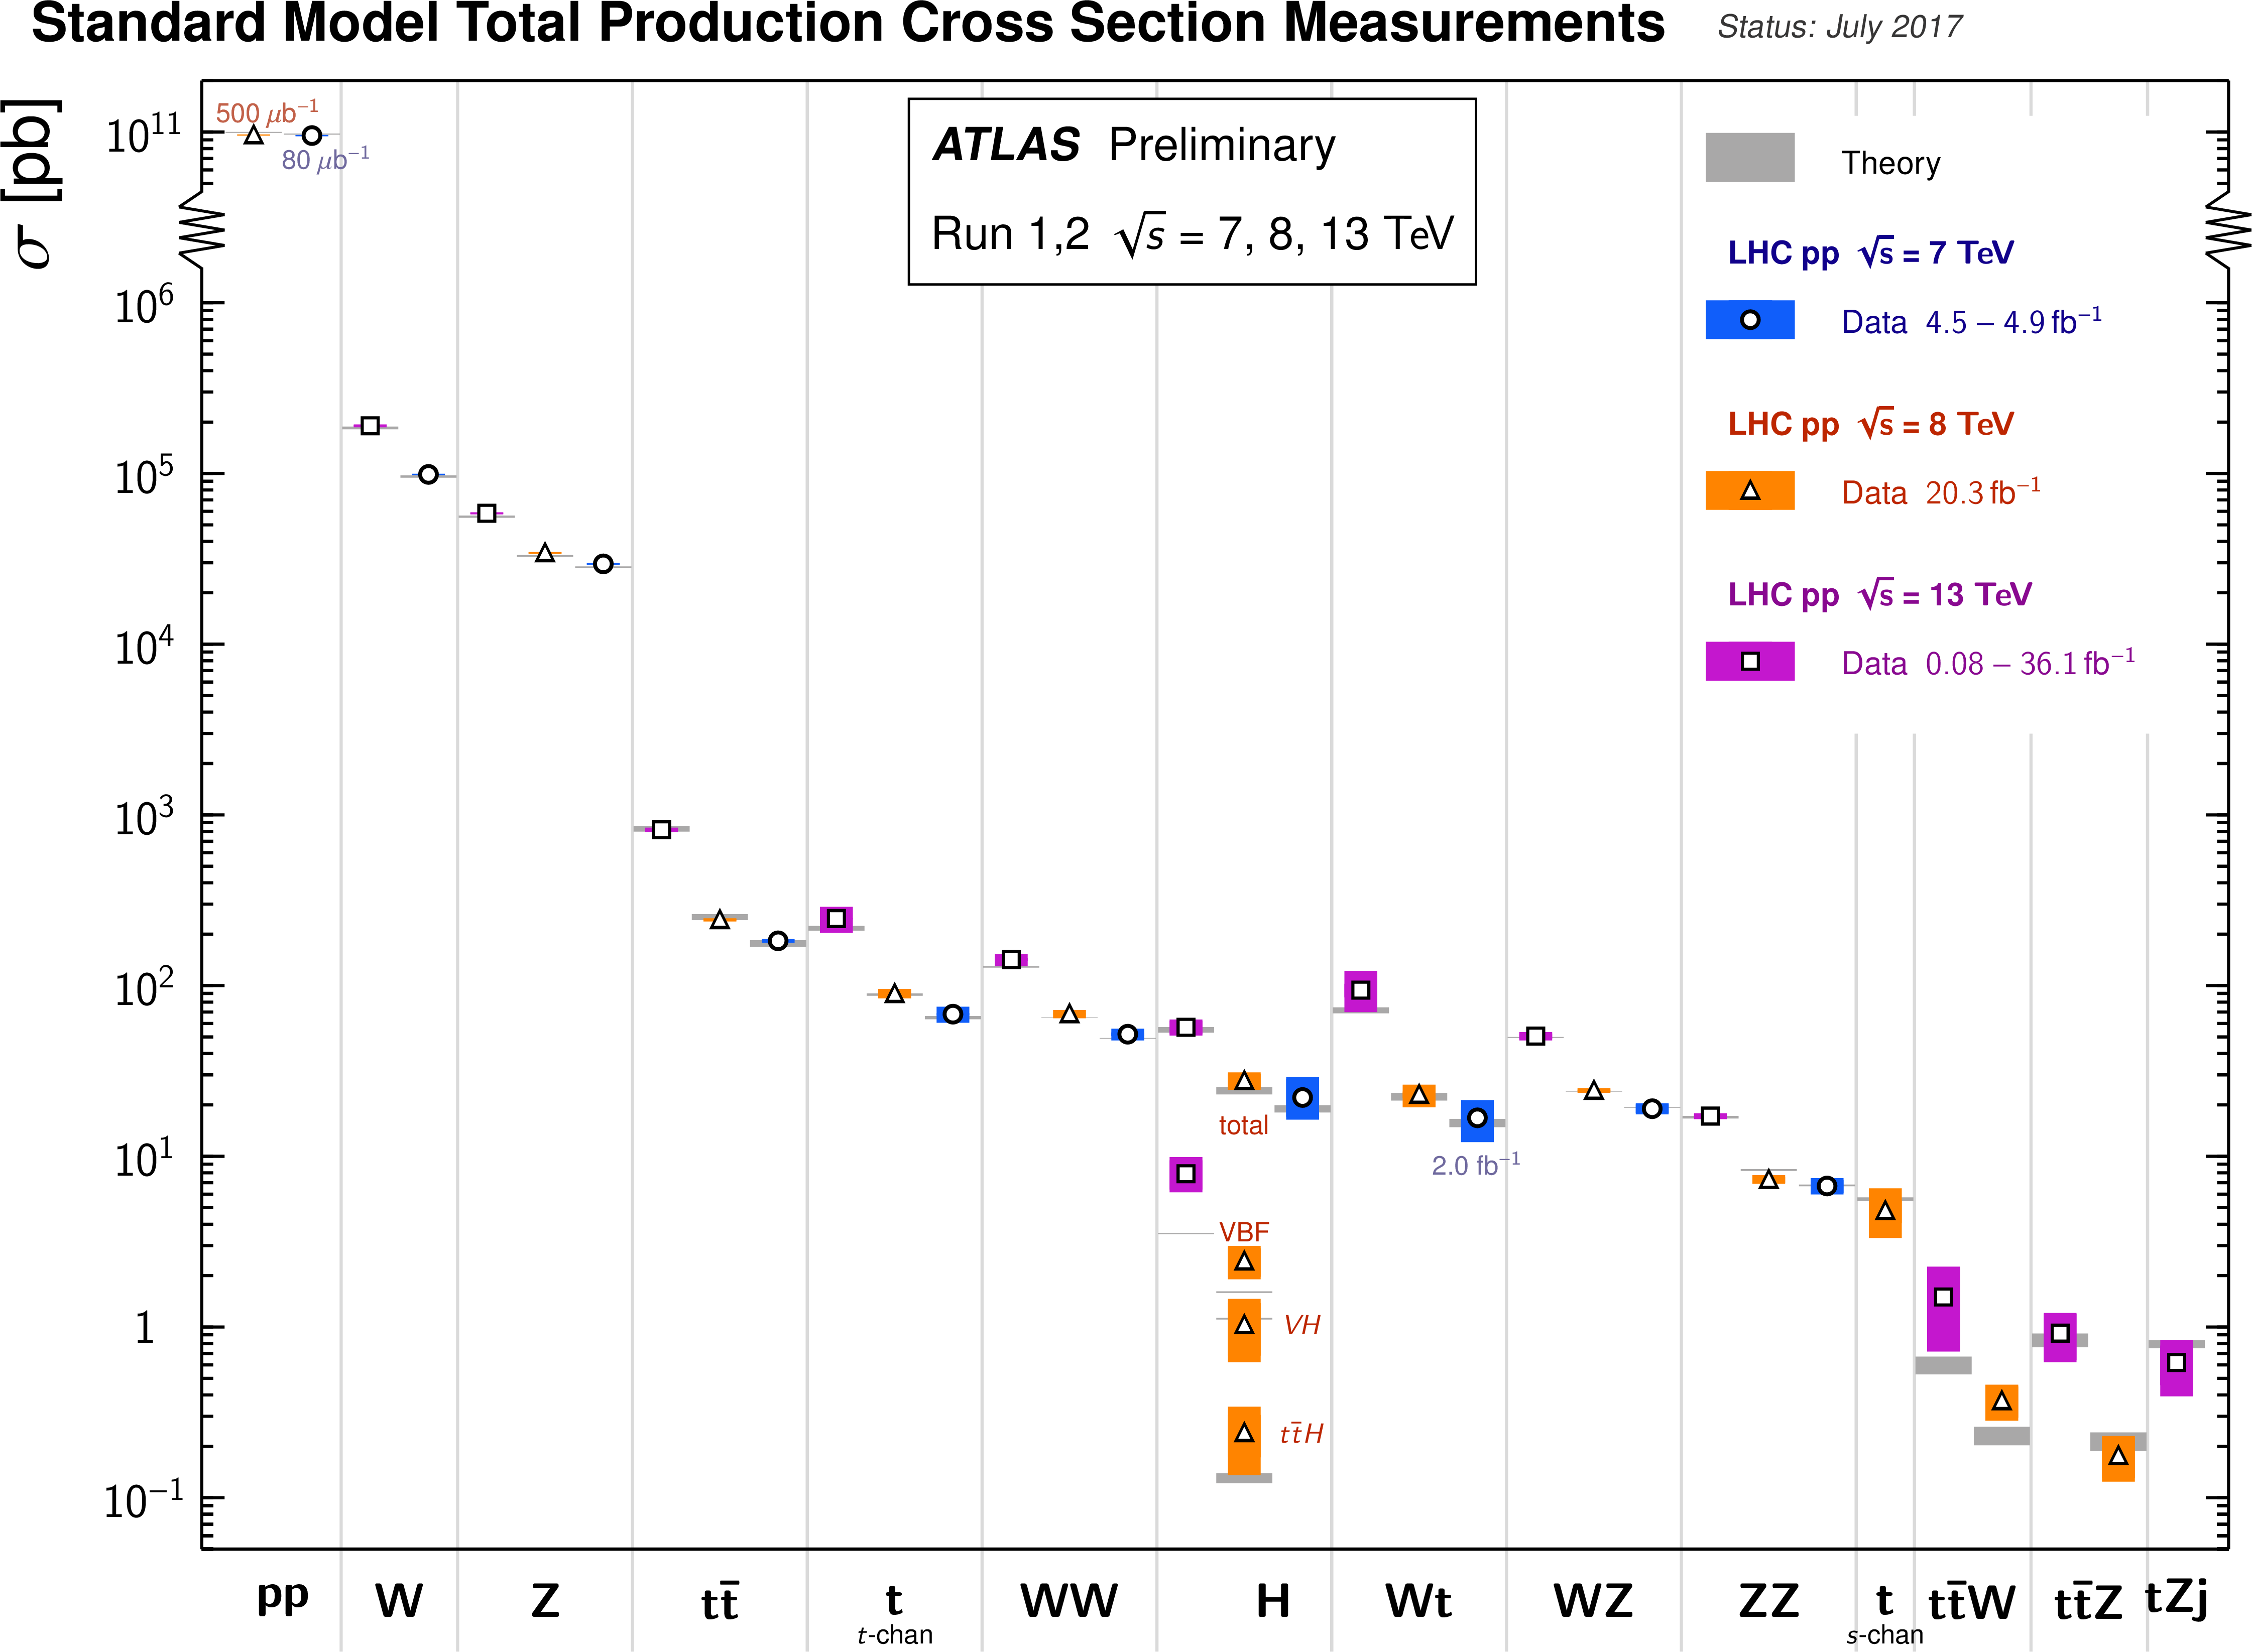
\includegraphics[width=\textwidth]{theory/ATLAS_a_SMSummary_TotalXsect}
			\caption{\label{fig:ATLAS_a_SMSummary_TotalXsect} Summary of several Standard Model total production cross section measurements, corrected for leptonic branching fractions, compared to the corresponding theoretical expectations. All theoretical expectations were calculated at NLO or higher. The luminosity used for each measurement is indicated close to the data point. Uncertainties for the theoretical predictions are quoted from the original ATLAS papers. They were not always evaluated using the same prescriptions for PDFs and scales. Not all measurements are statistically significant yet \cite{ATLAS_a_SMSummary_TotalXsect}.}
		\end{figure}



		\subsection*{Hierarchy Problem}

			The coupling of every particle to the Higgs field contributes to the mass of the Higgs field, $m_H^2$. In particular, The term due to fermionic loop coupling is given by:

			\begin{equation}
			\label{eq:mH_fermionic_contribution}
			\Delta m_H^2 = - \frac{\left | \lambda_f \right |^2}{8 \pi ^2} \Lambda_{\mathrm{UV}}^2 + \dots ,
			\end{equation}

			\noindent where $\Lambda_{\mathrm{UV}}$ is the ultraviolet momentum cut-off, selected as the cut-off value for the loop integral. If $\Lambda_{\mathrm{UV}}$ laid somewhere around the Planck scale ($\sim 2 \cdot 10^{18} \gev$), at which a QFT description of gravity is believed to become possible, then the correction to the Higgs mass would be around 30 orders of magnitude larger than Higgs mass itself. However, electroweak unification has been observed around $m_Z \sim O(100\gev)$ therefore, $m_H^2$ is not a natutal parameter. In other words, this difference between the electroweak scale and the Planck scale arisen from the quantum corrections to the Higgs mass is the so-called Hierarchy Problem \cite{Weinberg1976}.



		\subsection*{Neutrino Masses}

			The Super-Kamiokande Collaboration first, in 1998 \cite{SK1998}, and SNO Collaboration later, in 2001 \cite{SNO2001}, have provided measurements of the neutrino flux from solar and atmospheric sources. 
			The Nobel Prize in Physics 2015 was awarded jointly to Takaaki Kajita and Arthur B. McDonald ``for the discovery of neutrino oscillations, which shows that neutrinos have mass'' \cite{Nobel2015}. Such feature contraddicts the absence of a mechanism for mass generation for the neutrinos. 

			Various exotic solutions are on the market: one possible solution could be to add the so-called Majorana mass terms for the neutrino (seesaw mechanism). Neutrino physics could unveil physics beyond the SM.



		\subsection*{Dark Matter}

			Although dark matter (DM) has never been directly observed, its existence is inferred from its gravitational effects. For example, looking at galaxies rotation, it was observed that the rotation speed was higher than expected, given the amount of visible matter. Two different reasoning arose during the last century to justify such effect either there is matter that cannot be seen by us (in terms of visible light), which contributes to the galatcis mass; or the general relativity works differently at galactic distances. The former is believed to be the most likely and it implies the existence of new particles which do not interact via electromagnetic interaction, the so-called Weakly Interacting Massive Particles (WIMPs).





	\section{Supersymmetry}
	\label{sec:SUSY}

		SUperSYmmetry (SUSY) is a theory that links gravity with the other fundamental forces of nature by introducing a space-time symmetry that relates bosons to fermions and vice-versa, via a transformation of the form of:  

		\begin{equation}
		\label{eq:susy_transformation}
			Q \ket{\mathrm{fermion}} = \ket{\mathrm{boson}}, \qquad Q \ket{\mathrm{boson}} = \ket{\mathrm{fermion}}
		\end{equation}

		\noindent For each SM particle there exists a superparner (also referred to as \emph{sparticle}) with a spin difference of $\Delta s = 1/2$. As of today, superpartners have not been observed yet, resulting in the assumption that SUSY must be a broken symmetry, otherwise superpartners would have had the same quantum numbers and masses as their SM equivalent. However, if sparticles were to be too heavy the hierarchy problem would still remain unsolved. The \emph{soft} SUSY breaking mechanism overcomes this problem imposing contrains on the masses of sparticles to a range that can be experimentally explored.

		\subsection{Why SUSY?}
			
			bla

		\subsection{Minimal Supersymmetric Standard Model}
			
			bla

		\subsection{\emph{R}-parity SUSY}
		
			bla

		\subsection{Simplified models}
		
			bla


		\subsection{Phenomenological MSSM}
		
			bla

